Authors: Philipp Neumann\footnote{philipp.neumann@uni-hamburg.de}, Daniel Ruprecht\footnote{D.Ruprecht@leeds.ac.uk}, Martin Schreiber\footnote{M.Schreiber@exeter.ac.uk, Corresponding author}

This paragraph discusses a set of benchmarks which are suited to show the application of parallel-in-time methods to simulations based on the Navier-Stokes (NS) equations and the Lattice Boltzmann method (LBM).
Since the Lattice Boltzmann method resembles the Navier-Stokes equations asymptotically, we suggest benchmarks for both types of flow simulation.
We restrict considerations to incompressible (Navier-Stokes) and weakly compressible (Lattice Boltzmann) systems.


\subsubsection{Incompressible Navier-Stokes equations}
The two-dimensional incompressible Navier-Stokes equations can be formulated with (see \cite{wikiTaylorGreen}) the continuity equation
\begin{eqnarray}
\frac{\partial v_0}{\partial x_0}+ \frac{\partial v_1}{\partial x_1} &=& 0\\
\end{eqnarray}
and the momentum equations
% NOTE: Ich habe rho hier rausgeschmissen, da man die Dichte mE für die Szenarien nicht braucht.
\begin{eqnarray}
\frac{\partial v_0}{\partial t} + v_0\frac{\partial v_0}{\partial x_0} + v_1\frac{\partial v_0}{\partial x_1} &=&
-\frac{\partial p}{\partial x_0} + \nu \left( \frac{\partial^2 v_0}{\partial x_0^2} +
\frac{\partial^2 v_0}{\partial x_1^2} \right)\\
%
\frac{\partial v_1}{\partial t} + v_0\frac{\partial v_1}{\partial x_0} + v_1\frac{\partial v_1}{\partial x_1} &=&
-\frac{\partial p}{\partial x_1} + \nu \left( \frac{\partial^2 v_1}{\partial x_0^2} +
\frac{\partial^2 v_1}{\partial x_1^2} \right)
\end{eqnarray}



\subsubsection{Lattice Boltzmann model}
The Lattice Boltzmann method (LBM) is formulated at the mesoscopic level and can be positioned between the microscale simulations (e.g.\,molecular dynamics) and macroscopic simulations (e.g. Navier-Stokes).
Based on the Boltzmann distribution function, several discretization steps lead to a cellular-automaton formulation.
For PinT studies we restrict studies to two-dimensional formulations in this benchmark suite; three-dimensional studies are of significance, e.g. in the case of turbulent flows, and may be included at a later stage.
Using the DdQq notation with $d$ denoting the dimensions and $q$ the number of lattice vectors, the D2Q9 formulation may be used.
See e.g.\,\cite{korner2005lattice} for the following formulation.

For the D2Q9 model, the discrete set of propagation velocities are given by $\vec{v}_i = \vec{e}_i$ with $\vec{e}_i$ all possible lattice vectors with $j = |\vec{e}_i|^2 \in \{0,1,2\}$.
Here, $\vec{e}_0$ is the zero-vector which points to the local cell itself, $vec{e}_{\{1,2,3,4\}}$ the vectors pointing to the left, right, bottom, top adjacent cell and $vec{e}_{\{5,6,7,8\}}$ the diagonal oriented vectors pointing to the corner-adjacent cells.
Let $f_i(\vec{x})$ be the density distribution in cell $\vec{x}$ for lattice velocity $\vec{e}_i$, $t$ the simulation time, $t+1$ the parametrised time step size propagating bulks of particles from one cell along the lattice vectors and $F_i$ some external force; in the presented test cases, $F_i=0$ and can thus be omitted.
Given the density distributions $f_i$ of a cell along lattice vectors $\vec{e}_i$, we can compute the density $\rho$ and pressure $p$
\begin{eqnarray}
	\rho &=& \sum_{i=0}^q f_i\\
        p    &=& \cfrac{1}{3} \rho
\end{eqnarray}
and momentum
\begin{equation}
	\rho \vec{v} = \sum_{i=0}^q f_i \vec{e}_i
\end{equation}

The LB update rule is given by
\begin{equation}
	f_i(\vec{x}+\vec{e}_{i}, t+1) = f_i(\vec{x},t) - \frac{1}{\tau}
	\left(
		f_i(\vec{x},t) - f_i^{eq}(\vec{x},t)
	\right)
	+ F_i
\end{equation}
with equilibrium distribution
\begin{equation}
	f_i^{eq}(\rho, \vec{v}) = \omega_j \rho
	\left[
		1 + 3(\vec{e}_i \cdot \vec{v}) + \frac{9}{2} (\vec{e}_i \cdot \vec{v})^2 - \frac{3}{2} \vec{v}^2
	\right]
\end{equation}
where
	$\omega_0 = \frac{16}{36}$,
	$\omega_1 = \frac{4}{36}$ and
	$\omega_2 = \frac{1}{36}$.



\subsubsection{Benchmarks}

The suggested benchmarks LBM-1 and LBM-2 both have an analytical solution which makes them very well suited to test for convergence of PinT methods.

%For all benchmarks, the domain is given on the quad shaped domain $\Omega=[0;1]^2$ with a velocity profile $u(\vec{x})$ with $\vec{x} \in \Omega$ and boundary conditions $\vec{x} \in d\Omega$.


%%%%%%%%%%
%%% LBM-1: Couette flow
%%%%%%%%%%
\paragraph{LBM-1: Developing Couette Flow}

\subparagraph{Benchmark description}

We consider a channel setup with periodic conditions at the left and right boundary and a no-slip (e.g., half-way bounce back) boundary ($u(x_1=H,t)=0$, $t\geq 0$) at the top.
%\todo{Martin, you you may be have a sketch of the setup? Could be helpful to include. ANS: No, it's trivial :-)}
The bottom boundary moves at constant velocity $V=0.05$ towards the right, $u(x_1=0,t) = V$, $t\geq 0$.
The distance between bottom and top boundary is denoted by $H$.
The initial velocity field is set to zero everywhere inside the channel, pressure (and density, respectively) are set to a constant value; in LBM, $\rho=1$ everywhere.

Given this scenario, the incompressible Navier-Stokes system simplifies to~\cite{transientPlaneCouetteFlow}
\begin{eqnarray}
	\frac{\partial v_0}{\partial t} = \nu \frac{\partial^2 v_0}{\partial x_1^2}
\end{eqnarray}
and yields the analytic solution
$$
	v_0(x_1,t) = V\left(1 - \frac{x_1}{H} \right) - \frac{2V}{\pi}\sum_{k=1}^{\infty}\frac{1}{k}\sin\left(\frac{k\pi}{H} x_1\right)e^{-\frac{k^2\pi^2}{H^2}\nu t}.
$$
Pressure $p$ and velocity component $v_1$ remain constant/zero.




\subparagraph{PinT tests}

The results of applying a PinT method should include the following parameter ranges:

\begin{itemize}
	\item Domain resolution $N\times N$ with $N \in \{ 32, 64\}$
	\item Domain size $N \times N$ resulting in a mesh size $dx=1$ and $H=N$
	\item Viscosity: $\nu = 0.05$, velocity: $V=0.05$
	\item In case of using LBM, the Mega Lattice Updates per Second for the fine time stepping
\end{itemize}
As an alternative to the given domain size, appropriate re-scaling of all quantities to a unit square may be considered (e.g., for Navier-Stokes solvers).

PinT studies should be done with L1, L2 and Linf errors:
\begin{itemize}
	\item PinT studies should be done with $t \in \{ 10, 100, 1000 \}$\todo{Determine if these values make sense!}
	\item Using a PinT method: Convergence plots to solution over time at selected points in time.
\end{itemize}

\begin{figure}[t!]
\begin{tabular}{c c}
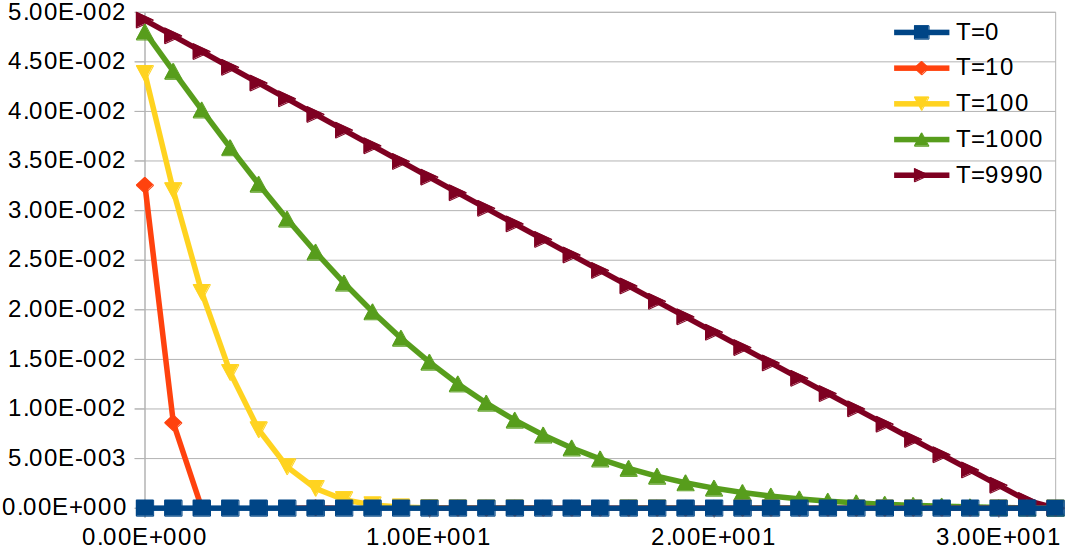
\includegraphics[width=0.45\textwidth]{lattice_boltzmann_and_navier_stokes_images/32x32_couette_v0.png} & 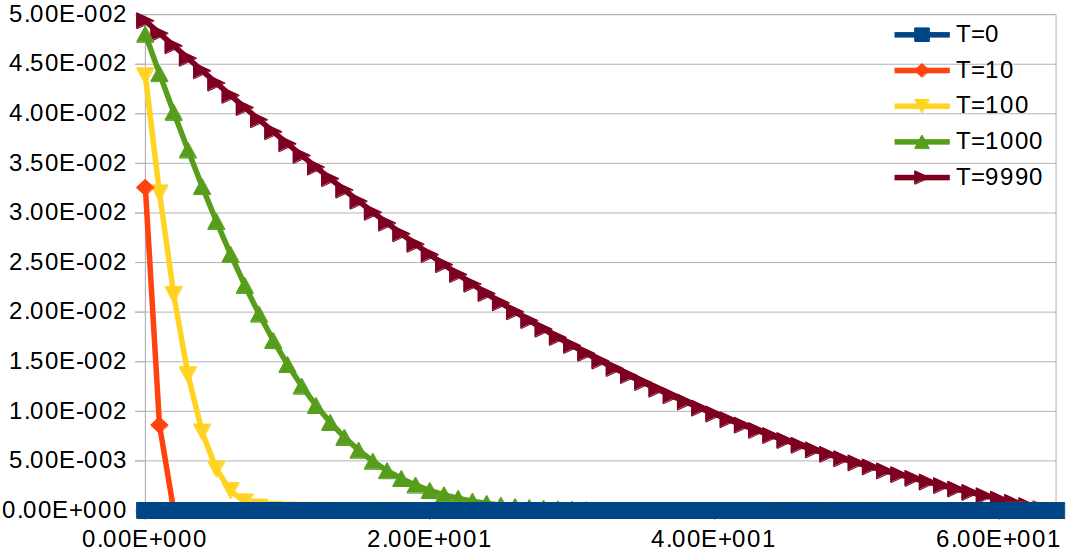
\includegraphics[width=0.45\textwidth]{lattice_boltzmann_and_navier_stokes_images/64x64_couette_v0.png}
\end{tabular}
\caption{Velocity profile $v_0(x_1)$ of LB-based Couette flow simulation across the channel at different instance in time $T$. Left: $N=32$. Right: $N=64$.}
\end{figure}

\todo{For PINT, we should probably ask for work-precision diagrams, that is plots showing error versus runtime? After all, we are all about computing the solution faster.}

%%%%%%%%%%
%%% LBM-2: Taylor Green
%%%%%%%%%%
\paragraph{LBM-2: Taylor Green}



\subparagraph{Benchmark description}

The Taylor Green benchmark assumes the incompressible Navier-Stokes equations, see \cite{taylor1937mechanism} for more information.
The setup consists of a periodic two-dimensional box of size $2\pi \times 2\pi$ with initial conditions for velocity field and pressure prescribed; for the initial conditions, see sections below.
The following equations and formulations are amongst others based on \cite{wikiTaylorGreen} and \cite{taylor1937mechanism}.


A particular solution of the velocity field over time is
\begin{eqnarray}
%	u = A \cos a x \sin b y \sin c z\\
%	v = B \sin a x \cos b y \sin c z\\
%	w = C \sin a x \sin b y \cos c z
% 2D formulation from WIKI
	v_0(x_0,x_1,t) &=& u_c\cos \left(2\pi x_0\right) \sin \left(2\pi x_1\right) F(t)\\
	v_1(x_0,x_1,t) &=& -u_c\sin \left(2\pi x_0\right) \cos \left(2\pi x_1\right) F(t)
\end{eqnarray}
%with the consistency requirement
%\begin{equation}
%	Aa + Bb + Cc = 0
%\end{equation}
with
$$
	F(t) = e^{-2\nu_c t}
$$
%A solution at time $t$ is then given by
%\begin{eqnarray}
%	u	&=&A(a-\theta vt) \cos ax \sin by \sin cz\\
%		& &+ \frac{A_3}{a} t \sin 2ax \cos 2by\\
%		& &- \frac{A_2}{a} t \sin 2ax \cos 2cz
%\end{eqnarray}

The solution of the pressure field is given by
\begin{eqnarray}
	p(x_0,x_1,t) &=& p_0-\frac{u_c^2}{4} \left( \cos \left(4\pi x_0\right) + \cos \left(4\pi x_1\right) \right) F^2(t)
\end{eqnarray}
with arbitrary constant $p_0$ (in the incompressible Navier-Stokes sense).
For LBM, we set $p_0:=\frac{1}{3}$.


\subparagraph{PinT tests}

The results of applying a PinT method should include the following parameter ranges:

\begin{itemize}
	\item Domain resolution $N\times N$ with $N \in \{ 32, 64\}$
	\item Domain size $2\pi\times 2\pi$ resulting in a mesh size $dx=2\pi/N$
	\item Viscosity in LB simulation: $\nu = 0.05$ (corresponding to relaxation time $\tau=0.65$ in the BGK model), $u_c = 0.01$; choosing the time step $dt\stackrel{!}{=}dx$, this corresponds to a viscosity value $\nu_c=\nu\cdot dx^2/dt \approx 0.00981747$. The (dimensionless) velocity and pressure values of the LB simulation and the analytic solution from above correspond to each other under this scaling. For Navier-Stokes simulations, a viscosity $\nu_c$ shall directly be used
	\item PinT studies should be done with $t \in \{ 10, 100, 1000 \}$
	\item In case of using LBM, the Mega Lattice Updates per Second for the fine time stepping
\end{itemize}
As an alternative to the given domain size, appropriate re-scaling of all quantities to a unit square may be considered (e.g., for Navier-Stokes solvers).

PinT studies should be done with L1, L2 and Linf errors:
\begin{itemize}
	\item Using a PinT method: Convergence plots to current solution.
\end{itemize}

\begin{figure}[t!]
\begin{tabular}{c c}
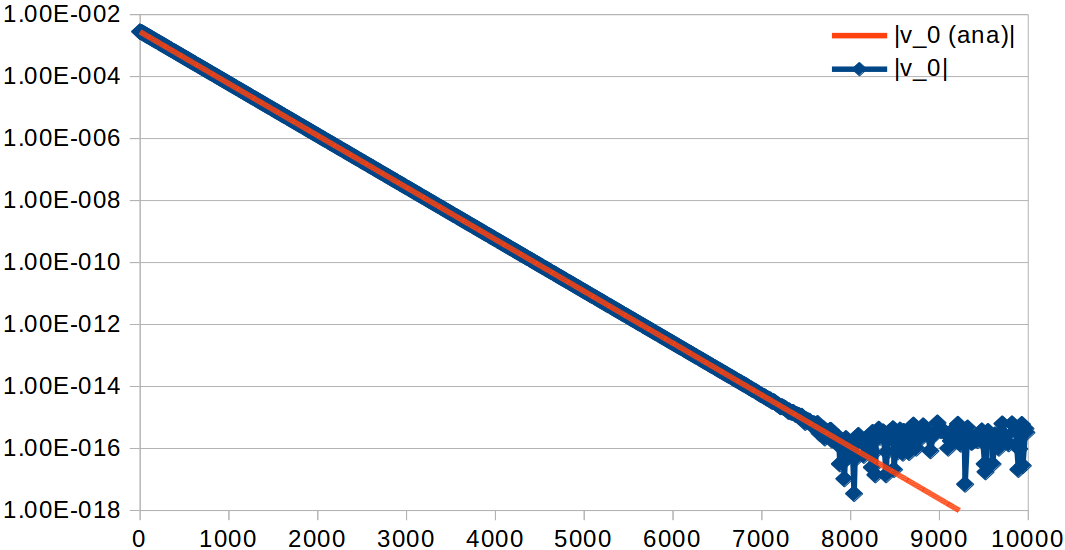
\includegraphics[width=0.45\textwidth]{lattice_boltzmann_and_navier_stokes_images/32x32_15x15_taylorgreen_v0.png} & 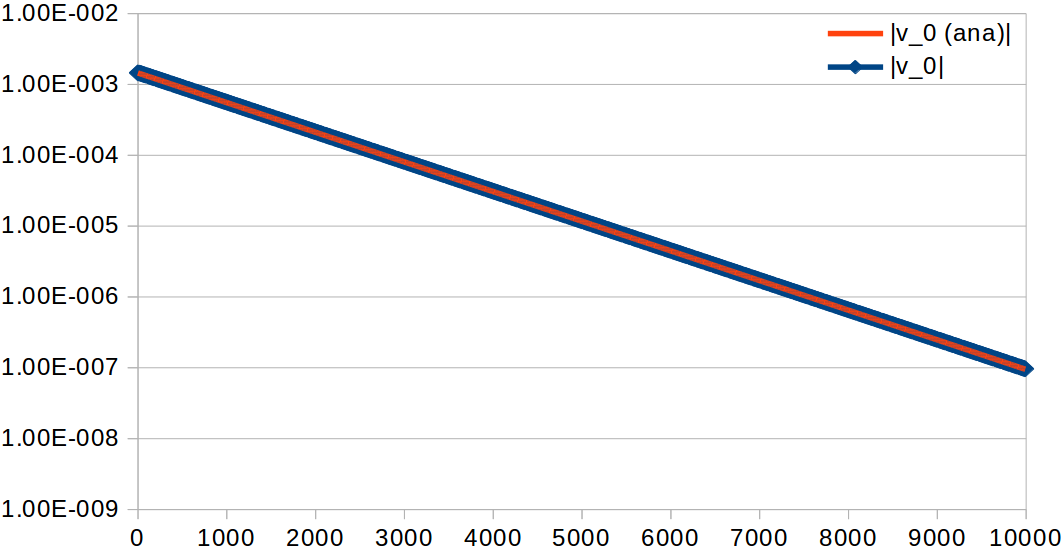
\includegraphics[width=0.45\textwidth]{lattice_boltzmann_and_navier_stokes_images/64x64_31x31_taylorgreen_v0.png}\\
(a) & (b)\\
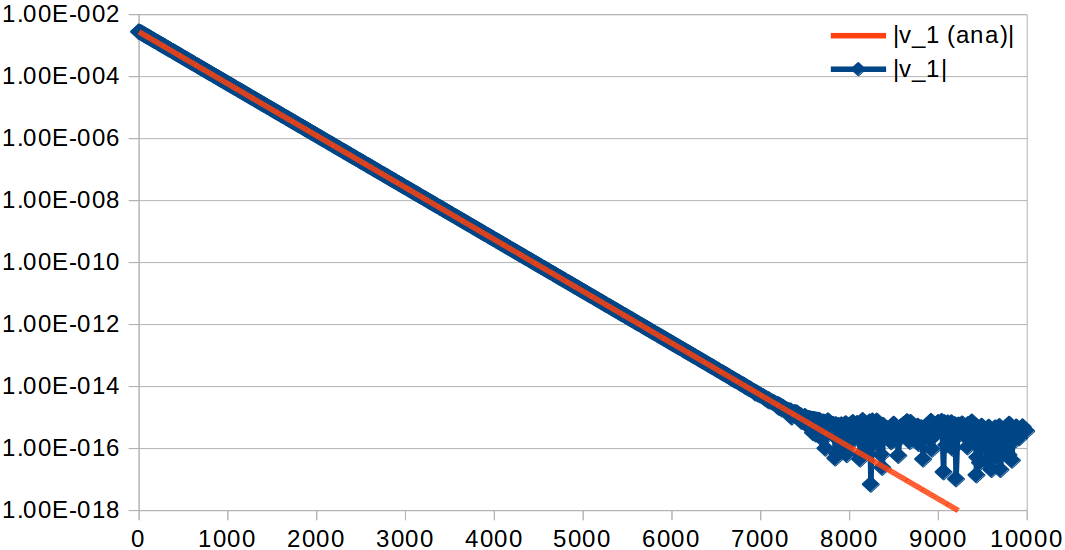
\includegraphics[width=0.45\textwidth]{lattice_boltzmann_and_navier_stokes_images/32x32_15x15_taylorgreen_v1.png} & 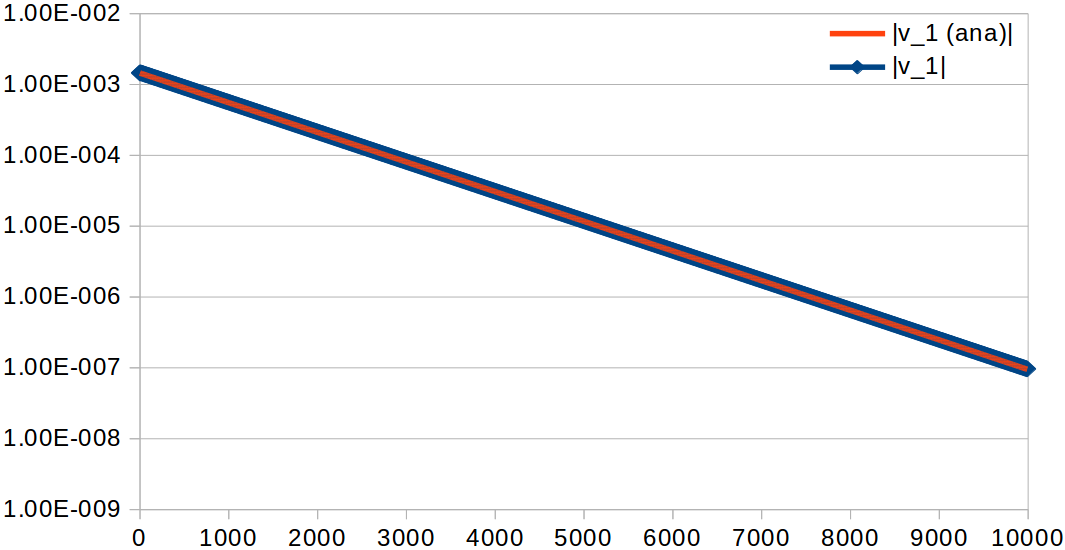
\includegraphics[width=0.45\textwidth]{lattice_boltzmann_and_navier_stokes_images/64x64_31x31_taylorgreen_v1.png}\\
(c) & (d)\\
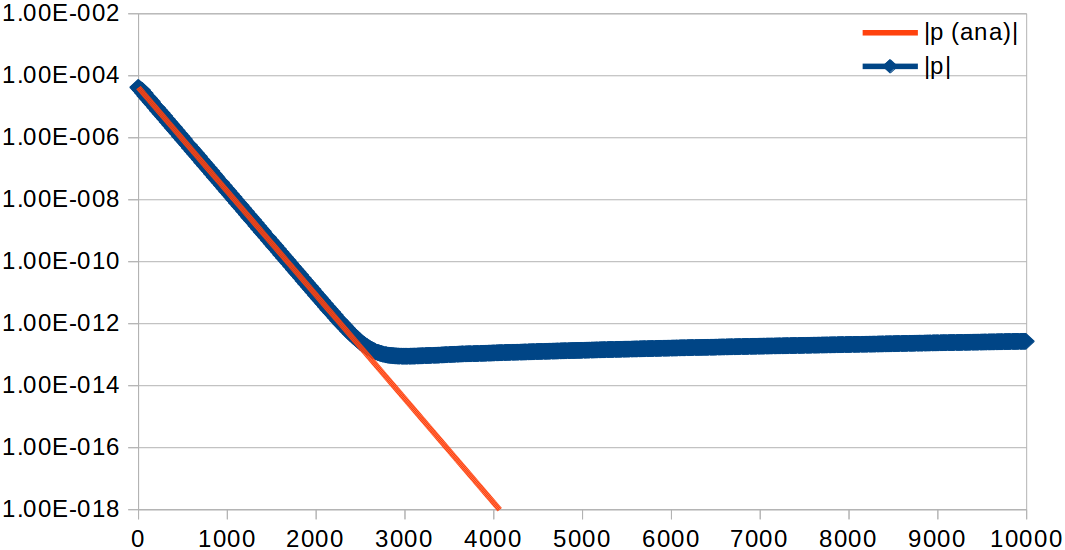
\includegraphics[width=0.45\textwidth]{lattice_boltzmann_and_navier_stokes_images/32x32_15x15_taylorgreen_p.png} & 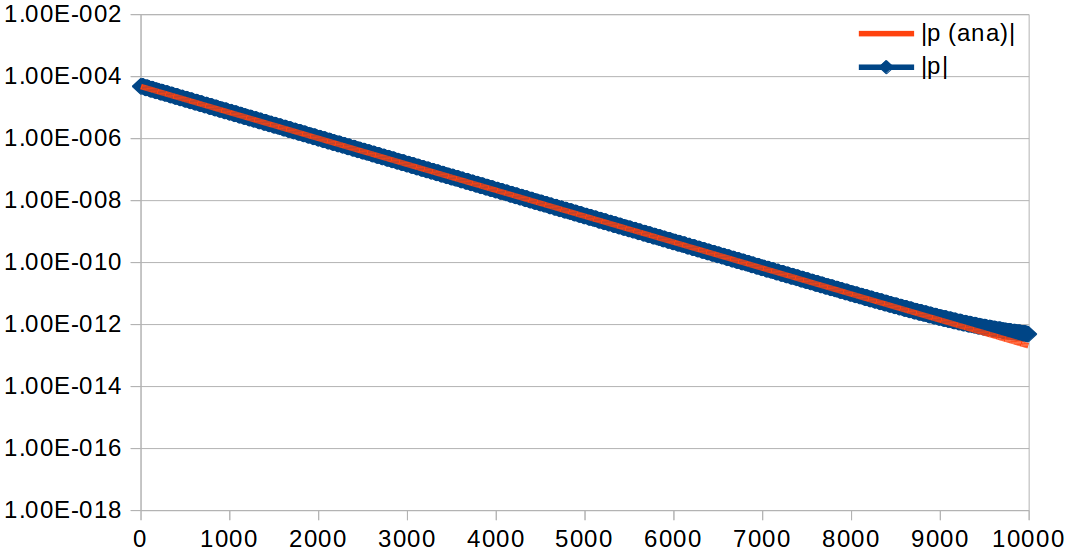
\includegraphics[width=0.45\textwidth]{lattice_boltzmann_and_navier_stokes_images/64x64_31x31_taylorgreen_p.png}\\
(e) & (f)
\end{tabular}
\caption{Taylor-Green solution for pressure and velocity over time interval $t\geq 10~000$. Left: solution measured in cell (15,15) corresponding to $(x_0,x_1)=(2.847,2.847)$ using $N=32$ cells in both x- and y-direction. Right: solution measured in cell (31,31) corresponding to $(x_0,x_1)=(2.994,2.994)$ using $N=64$ cells in both x- and y-direction. The blue lines correspond to the LB simulation, the red lines denote the analytic solution.}
\end{figure}

%%%%%%%%%%
%%% LBM-3: Driven Cavity
%%%%%%%%%%


%\subsection{LBM-3: Driven Cavity}
%
%\subsubsection{Benchmark description}
%
%\begin{figure}
%	\center
%	\includegraphics[width=0.6\textwidth]{pics_external/cavity_flow.png}
%	\caption{Driven cavity configuration, source: \cite{ghia1982high}}
%\end{figure}
%
%\begin{itemize}
%	\item Resolutions: $151^2$, $121^2$?!?
%	\item Reynolds numbers: 10000, 1000, 100?
%\end{itemize}
%
%\subsubsection{Reference solution}
%
%The reference solution is generated with standard fine time stepping.
%
%\subsubsection{PinT tests}
%
%The results of applying a PinT method should include the following parameter ranges:
%\todo{TODO}
%\begin{tabular}{cc}
%\end{tabular}

